%% ------------------------------------------------------------------------- %%
\chapter{Desenvolvimentos}
\label{cap:desenvolvimentos}

Embora neste exemplo tenhamos apenas um cap�tulo,  entre a introdu��o
e a conclus�o de uma monografia podemos ter uma sequ�ncia de cap�tulos
descrevendo o trabalho e os resultados. Estes podem descrever
fundamentos, trabalhos relacionados, m�todo/modelo/algoritmo proposto,
experimentos realizados, resulatdos obtidos.

Cada cap�tulo pode ser organizado em se��es, que por sua vez pode
conter subse��es.

Um exemplo de figura est� na figura~\ref{fig:graph}.
\begin{figure}[htb]
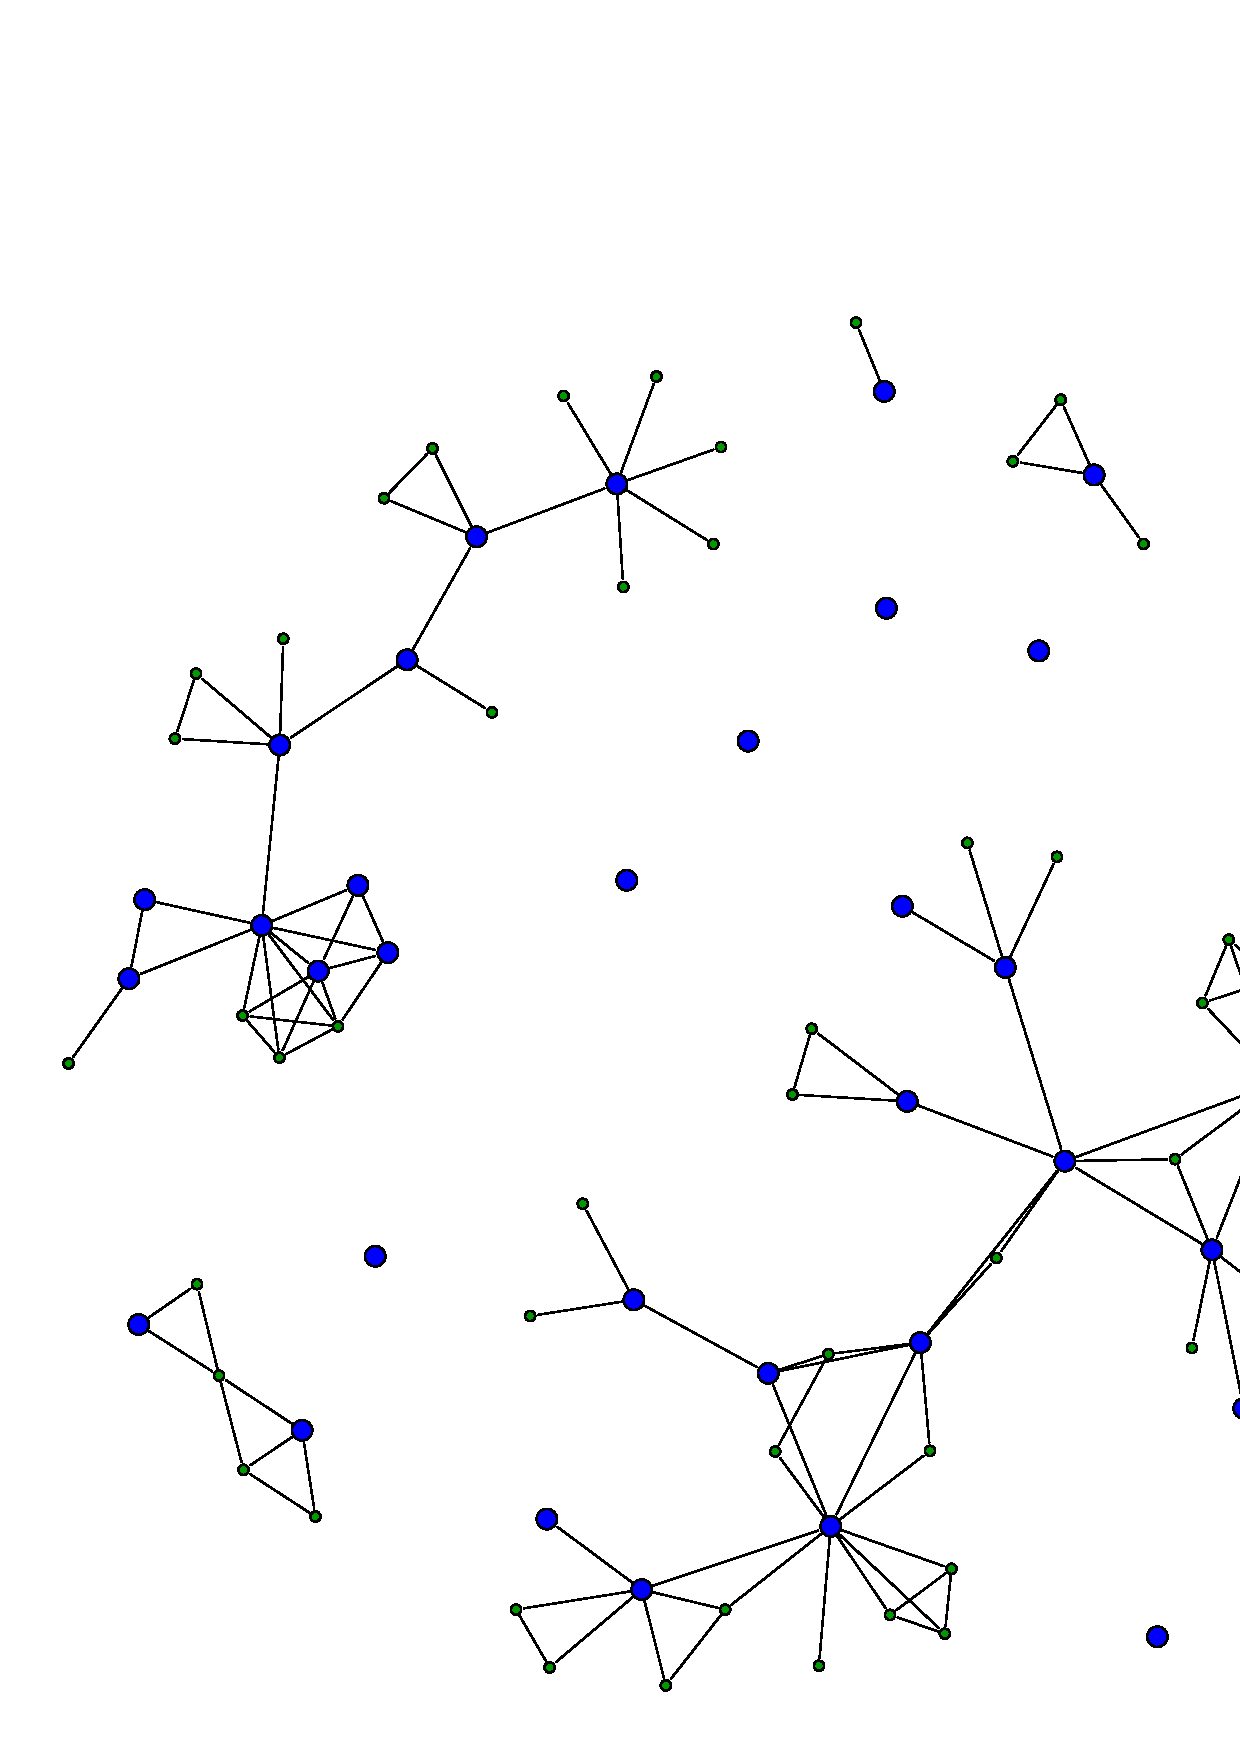
\includegraphics[width=5cm]{figuras/graph}
\caption{\label{fig:graph}Exemplo de uma figura.}
\end{figure}
%\chapter{Gerando imagens de cartas no android}
%\label{cap:desenvolvimentos}
% O objetivo deste cap�tulo � expor as t�cnicas e decis�es para gerar as imagens das cartas no
% celular

% Introduzir aos conceitos b�sicos de imagens, perspectiva, vis�o e objetos em rela��o � conputa��o
% gr�fica, as tecnologias como biblioteca gr�fica e bibliotecas do android para desenvolvimento de
% aplicativos

% Explicar as decis�es tomadas no desenvolvimento do GL(biblioteca gr�fica no aplicativo). Explicar
% as abstra��es que foram feitas para obter o GL.

% Mostras testes de experimento de tempo durante o processo de otimiza��o.